\definecolor{plot_orange}{rgb}{1, 0.639, 0}
\definecolor{plot_red}{rgb}{0.973, 0.463, 0.427}
\definecolor{plot_blue}{rgb}{0.153, 0.682, 0.937}
\definecolor{plot_green}{rgb}{0, 0.729, 0.22}
\definecolor{plot_gray}{rgb}{0.4, 0.4, 0.4}

In this chapter, we compare five different methods—Sparse, SQL Einsum, Torch, Legacy Sparse 
Einsum, and Sparse Einsum—on different problems. First, we compare them on various random
tensor hypernetworks and then, we evaluate their performance on five instances of the ``Einsum
Benchmark" \cite{einsum_benchmark} dataset.

\section{Random Tensor Hypernetworks}
In this section, we look at five different methods—Sparse, SQL Einsum, Torch, Legacy Sparse 
Einsum, and Sparse Einsum—on tensor sizes ranging from small to large. We generate Einsum 
problems by computing random tensor hypernetworks with a single varying parameter for each 
experiment. For each change of a parameter the results are evaluated using 10 differently 
seeded random tensor hypernetworks generated with identical parameters. We then evaluate 
each methods performance on the problem 10 times to get an average it/s.
\\
\\
First, we generate problems where we vary the maximum size of dimensions from 2 to 8. 
Figure \ref{fig:exp:max_dim_size} shows the performance for the different dimension sizes. 
The performance of all methods naturally decreases when the size of dimensions grows. However, 
the rate of this degradation differs significantly between the methods.

\begin{figure}[H]
    \centering
    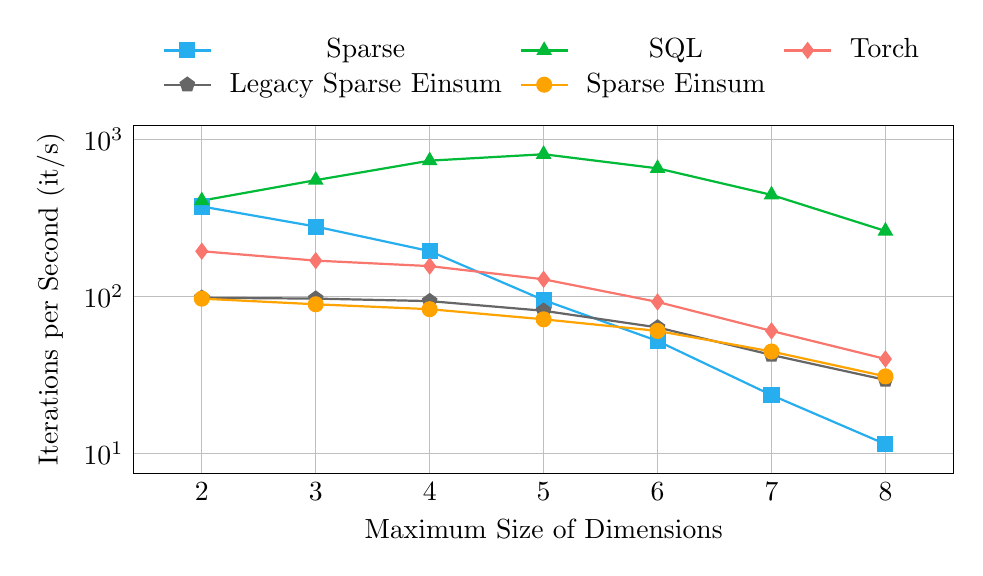
\begin{tikzpicture}
        \begin{axis}[
            xlabel={Maximum Size of Dimensions},
            ylabel={Iterations per Second (it/s)},
            grid=major,
            mark size=2.5pt,
            width=12cm,
            height=6cm,
            enlargelimits=0.1,
            xtick style={draw=none},  % Remove x-axis tick marks
            ytick style={draw=none},  % Remove y-axis tick marks
            ymode=log,                % Logarithmic scale for y-axis
            log basis y=10,           % Set base 10 for y-axis
            legend style={
                at={(0.5,1.05)}, % Position above the plot
                anchor=south, % Anchor to the south of the legend
                legend columns=3, % Arrange entries side by side
                column sep=1ex, % Space between columns
                draw=none, % Remove the border
                fill=none, % Remove the background fill
            }
        ]
    
        % Sparse (Square marker)
        \addplot[
            color=plot_blue,
            mark=square*,
            thick
        ] coordinates {
            (2, 373.779) (3, 278.362) (4, 194.133) (5, 94.575)
            (6, 51.880) (7, 23.436) (8, 11.405)
        };
        \addlegendentry{Sparse}
    
        % SQL (Triangle marker)
        \addplot[
            color=plot_green,
            mark=triangle*,
            thick
        ] coordinates {
            (2, 407.201) (3, 550.046) (4, 732.296) (5, 804.534)
            (6, 654.144) (7, 442.977) (8, 260.772)
        };
        \addlegendentry{SQL}
    
        % Torch (Diamond marker)
        \addplot[
            color=plot_red,
            mark=diamond*,
            thick
        ] coordinates {
            (2, 193.741) (3, 168.812) (4, 155.748) (5, 128.345)
            (6, 92.042) (7, 60.147) (8, 39.834)
        };
        \addlegendentry{Torch}
    
        % Legacy_Sparse_Einsum (Pentagon marker)
        \addplot[
            color=plot_gray,
            mark=pentagon*,
            thick
        ] coordinates {
            (2, 97.820) (3, 96.657) (4, 93.159) (5, 80.838)
            (6, 63.319) (7, 42.265) (8, 29.298)
        };
        \addlegendentry{Legacy Sparse Einsum}
        
        % Sparse_Einsum (Circle marker)
        \addplot[
            color=plot_orange,
            mark=*,
            thick
        ] coordinates {
            (2, 96.587) (3, 88.914) (4, 82.745) (5, 71.318)
            (6, 60.150) (7, 44.452) (8, 30.854)
        };
        \addlegendentry{Sparse Einsum}
    
        \end{axis}
    \end{tikzpicture}
    \caption{Performance of different methods vs maximum size of the dimensions. The plot 
    shows the number of iterations per second for each method across varying dimension sizes.}
    \label{fig:exp:max_dim_size}
\end{figure}

\noindent
Sparse performance decreases quickly when the maximum number of dimensions that the tensors 
can have increases. It has the steepest decline of all the methods. In general, SQL Einsum is 
superior for larger maximum sizes of dimensions, although it also declines more steeply in 
comparison with both Sparse Einsum implementations and Torch, which are much more constant 
in performance. The SQL implementations iterations per second rise, when the maximum size 
of dimensions increases from 2 to 5 and from thereon decreases constantly with rising possible 
sizes for the dimensions. Sparse Einsum and the legacy version of Sparse Einsum demonstrated 
very similar trends, though the legacy variant was a little better at most dimension sizes 
than the newer implementation. This is likely due to the additional overhead introduced by 
parallelization, which only pays of when computing large, sparse tensors.
\\
The results of Figure \ref{fig:exp:max_num_dim} illustrate how the computational performance 
of each method varies with increasing dimensionality in tensor hypernetworks. Sparse shows a 
rapid decline as dimensionality increases, becoming inefficient at higher dimensions. SQL 
Einsum exhibits an unusual pattern, performing poorly at low and high dimensions but peaking 
in the middle range. Torch remains relatively stable, handling dimensionality increases 
consistently well. Sparse Einsum initially declines but improves at higher dimensions, 
indicating resilience to complexity. Legacy Sparse Einsum follows a similar trend, with fairly 
stable performance across different dimensions, excelling at moderate to high dimensionality. 
Overall, Torch, Sparse Einsum, and Legacy Sparse Einsum handle the increasing dimensionality 
best, while SQL Einsum performs optimally at intermediate dimensions, and Sparse struggles the 
most with larger networks.

\begin{figure}[H]
    \centering
    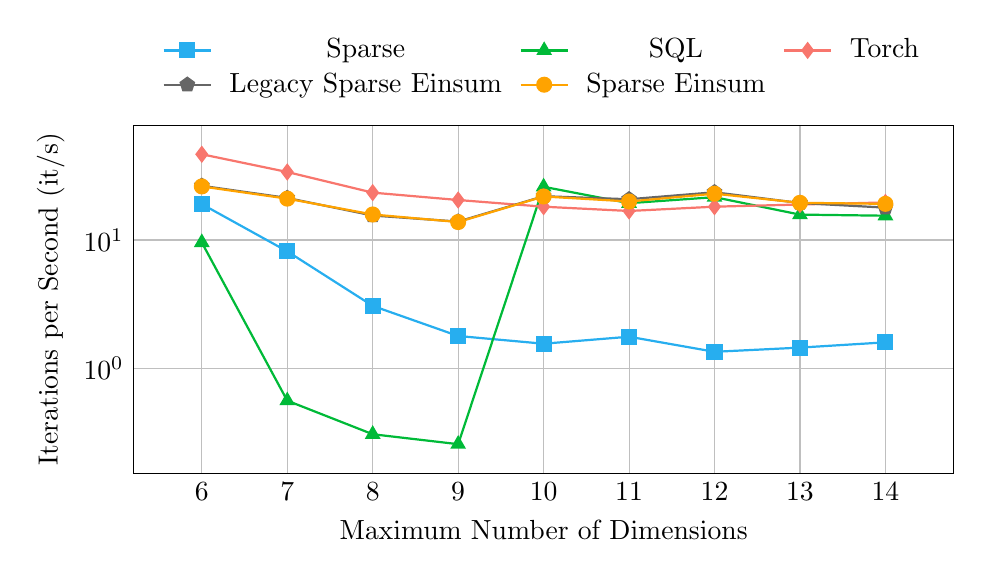
\begin{tikzpicture}
        \begin{axis}[
            xlabel={Maximum Number of Dimensions},
            ylabel={Iterations per Second (it/s)},
            grid=major,
            mark size=2.5pt,
            width=12cm,
            height=6cm,
            enlargelimits=0.1,
            xtick style={draw=none},  % Remove x-axis tick marks
            ytick style={draw=none},  % Remove y-axis tick marks
            ymode=log,                % Logarithmic scale for y-axis
            log basis y=10,           % Set base 10 for y-axis
            legend style={
                at={(0.5,1.05)}, % Position above the plot
                anchor=south, % Anchor to the south of the legend
                legend columns=3, % Arrange entries side by side
                column sep=1ex, % Space between columns
                draw=none, % Remove the border
                fill=none, % Remove the background fill
            }
        ]
    
        % Sparse_Time (Square marker)
        \addplot[
            color=plot_blue,
            mark=square*,
            thick
        ] coordinates {
            (6, 19.042) (7, 8.157) (8, 3.065) (9, 1.785) (10, 1.554)
            (11, 1.762) (12, 1.344) (13, 1.449) (14, 1.593)
        };
        \addlegendentry{Sparse}
    
        % SQL_Time (Triangle marker)
        \addplot[
            color=plot_green,
            mark=triangle*,
            thick
        ] coordinates {
            (6, 9.566) (7, 0.559) (8, 0.306) (9, 0.256) (10, 25.985)
            (11, 19.361) (12, 21.572) (13, 15.773) (14, 15.464)
        };
        \addlegendentry{SQL}
    
        % Torch_Time (Diamond marker)
        \addplot[
            color=plot_red,
            mark=diamond*,
            thick
        ] coordinates {
            (6, 46.602) (7, 33.894) (8, 23.399) (9, 20.497) (10, 18.177)
            (11, 16.834) (12, 18.184) (13, 18.909) (14, 19.625)
        };
        \addlegendentry{Torch}
    
        % Legacy_Sparse_Einsum_Time (Pentagon marker)
        \addplot[
            color=plot_gray,
            mark=pentagon*,
            thick
        ] coordinates {
            (6, 26.457) (7, 21.267) (8, 15.515) (9, 13.920) (10, 21.946)
            (11, 20.780) (12, 23.553) (13, 19.427) (14, 17.876)
        };
        \addlegendentry{Legacy Sparse Einsum}
        
        % Sparse_Einsum_Time (Circle marker)
        \addplot[
            color=plot_orange,
            mark=*,
            thick
        ] coordinates {
            (6, 26.151) (7, 21.004) (8, 15.809) (9, 13.802) (10, 21.840)
            (11, 19.967) (12, 22.961) (13, 19.494) (14, 19.137)
        };
        \addlegendentry{Sparse Einsum}
    
        \end{axis}
    \end{tikzpicture}
    \caption{Performance of different methods as a function of the maximum number of 
    dimensions. The plot shows the number of iterations per second for each method.}
    \label{fig:exp:max_num_dim}
\end{figure}

\noindent
The plots in Figure \ref{fig:exp:num_tensors} show each method's performance as the number 
of tensors increases. Sparse starts off highest but declines sharply as the number of tensors 
grows, eventually becoming among the slowest methods. SQL Einsum is competitive at the start 
but also has a large drop-off. However, Torch displays stable performance, gradually 
decreasing but remaining more efficient at higher tensor counts than Sparse and SQL. 
Sparse Einsum and Legacy Sparse Einsum started of lower than the other methods but perform 
much better than the others as the number of tensors increases. Both Sparse Einsum versions 
end up with slightly more iterations per second than Torch for larger number of tensors. 
SQL and Sparse show by far the largest performance degradation.

\begin{figure}[H]
    \centering
    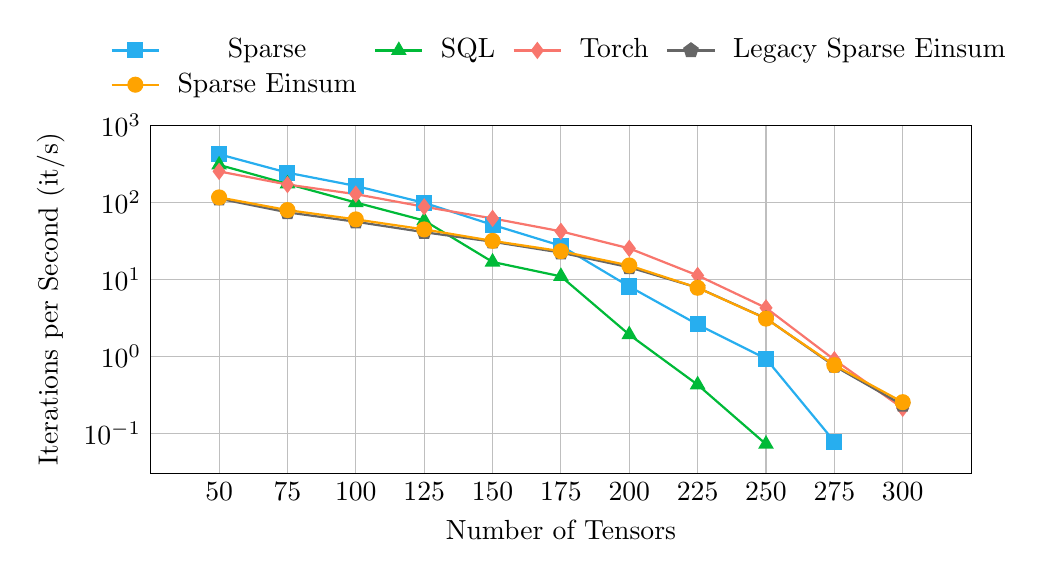
\begin{tikzpicture}
        \begin{semilogyaxis}[
            xlabel={Number of Tensors},
            ylabel={Iterations per Second (it/s)},
            grid=major,
            mark size=2.5pt,
            width=12cm,
            height=6cm,
            enlargelimits=0.1,
            xtick style={draw=none},
            ytick style={draw=none},
            xtick={50, 75, 100, 125, 150, 175, 200, 225, 250, 275, 300},
            xticklabels={50, 75, 100, 125, 150, 175, 200, 225, 250, 275, 300},
            legend style={
                at={(0.5,1.05)}, % Position above the plot
                anchor=south, % Anchor to the south of the legend
                legend columns=4, % Arrange entries side by side
                column sep=1ex, % Space between columns
                draw=none, % Remove the border
                fill=none, % Remove the background fill
            }
        ]
    
        % Sparse_Time (Square marker)
        \addplot[
            color=plot_blue,
            mark=square*,
            thick
        ] coordinates {
            (50, 421.397) (75, 243.002) (100, 163.534) (125, 98.735)
            (150, 51.171) (175, 27.372) (200, 8.103) (225, 2.608) 
            (250, 0.937) (275, 0.079)
        };
        \addlegendentry{Sparse}
    
        % SQL_Time (Triangle marker)
        \addplot[
            color=plot_green,
            mark=triangle*,
            thick
        ] coordinates {
            (50, 306.391) (75, 174.003) (100, 99.646) (125, 58.171)
            (150, 16.880) (175, 10.975) (200, 1.923) (225, 0.431) (250, 0.073)
        };
        \addlegendentry{SQL}
    
        % Torch_Time (Diamond marker)
        \addplot[
            color=plot_red,
            mark=diamond*,
            thick
        ] coordinates {
            (50, 252.421) (75, 170.495) (100, 127.919) (125, 87.753)
            (150, 62.042) (175, 42.147) (200, 25.338) (225, 11.279) 
            (250, 4.282) (275, 0.910) (300, 0.213)
        };
        \addlegendentry{Torch}
    
        % Legacy_Sparse_Einsum_Time (Pentagon marker)
        \addplot[
            color=plot_gray,
            mark=pentagon*,
            thick
        ] coordinates {
            (50, 111.878) (75, 74.319) (100, 56.124) (125, 41.069)
            (150, 30.887) (175, 22.307) (200, 14.387) (225, 7.829) 
            (250, 3.128) (275, 0.754) (300, 0.235)
        };
        \addlegendentry{Legacy Sparse Einsum}
        
        % Sparse_Einsum_Time (Circle marker)
        \addplot[
            color=plot_orange,
            mark=*,
            thick
        ] coordinates {
            (50, 116.182) (75, 79.501) (100, 60.205) (125, 44.611)
            (150, 31.703) (175, 23.280) (200, 15.195) (225, 7.810) 
            (250, 3.105) (275, 0.774) (300, 0.256)
        };
        \addlegendentry{Sparse Einsum}
    
        \end{semilogyaxis}
    \end{tikzpicture}
    \caption{Performance of different methods as a function of the number of tensors. We stop 
    the calculation early when a methods last data point is at less than 0.1 it/s.}
    \label{fig:exp:num_tensors}
\end{figure}